\documentclass[aspectratio=169,11pt]{beamer}

% Theme and colors
\usetheme{Madrid}
\usecolortheme{whale}
\setbeamertemplate{navigation symbols}{}
\setbeamertemplate{footline}[frame number]

% Packages
\usepackage[utf8]{inputenc}
\usepackage[T1]{fontenc}
\usepackage{graphicx}
\usepackage{booktabs}
\usepackage{amsmath}
\usepackage{hyperref}
\usepackage{tikz}
\usetikzlibrary{shapes,arrows,positioning,calc,fit,backgrounds}
\usepackage{siunitx}

% Bibliography
\usepackage[backend=biber,style=ieee,sorting=none]{biblatex}
\addbibresource{references.bib}

% Title information
\title[EECE5155 -- Module 4]{Module 4: Data Communication}
\author{Eduardo Baena}
\date{Spring 2026}
\institute{Northeastern University\\Department of Electrical and Computer Engineering\\
\texttt{e.baena@northeastern.edu}}

\begin{document}

%==============================================================================
% SLIDE 1: Title
%==============================================================================
\begin{frame}
    \titlepage
    \begin{center}
        \textbf{EECE5155: Wireless Sensor Networks and the Internet of Things}
    \end{center}
\end{frame}

%==============================================================================
% AI-NATIVE COURSE SECTION
%==============================================================================

\begin{frame}{This is an AI-Native Course}
    \begin{center}
        \Large
        \textbf{What does ``AI-native'' mean?}
    \end{center}
    
    \vspace{0.5cm}
    \textbf{AI tools are integrated into the workflow, not banned:}
    \begin{itemize}
        \item You \textbf{may} use GitHub Copilot, ChatGPT, Claude, etc.
        \item AI assistants can help you code faster \cite{peng2023impact}
        \item But the \textbf{responsibility} remains yours
    \end{itemize}
    
    \vspace{0.3cm}
    \begin{alertblock}{Key Principle}
        AI is a \textbf{tool}, not a replacement for understanding.
    \end{alertblock}
\end{frame}

\begin{frame}{Being an Engineer in 2026}
    \textbf{The landscape has changed:}
    
    \vspace{0.3cm}
    \begin{columns}[T]
        \begin{column}{0.48\textwidth}
            \textbf{What AI can do:}
            \begin{itemize}
                \item Generate boilerplate code
                \item Suggest implementations
                \item Find syntax errors
                \item Explain concepts
                \item Speed up development \cite{kalliamvakou2024measuring}
            \end{itemize}
        \end{column}
        \begin{column}{0.48\textwidth}
            \textbf{What AI cannot do:}
            \begin{itemize}
                \item Understand your requirements
                \item Verify correctness
                \item Take responsibility
                \item Debug hardware
                \item Sign off on safety
            \end{itemize}
        \end{column}
    \end{columns}
    
    \vspace{0.3cm}
    \begin{block}{Reality Check}
        AI-generated code can have subtle bugs \cite{siddiq2024quality}. \textbf{You must verify.}
    \end{block}
\end{frame}

\begin{frame}{Your Responsibility as an Engineer}
    \begin{center}
        \Large
        \textbf{You are accountable for everything you submit.}
    \end{center}
    
    \vspace{0.5cm}
    \textbf{This means:}
    \begin{enumerate}
        \item \textbf{Understand} every line of code you use
        \item \textbf{Verify} AI-generated outputs against specifications
        \item \textbf{Test} thoroughly -- AI doesn't test for you
        \item \textbf{Document} your design decisions (not AI's)
        \item \textbf{Defend} your work in oral examination
    \end{enumerate}
    
    \vspace{0.3cm}
    \begin{alertblock}{Professional Standard}
        ``The AI suggested it'' is \textbf{not} a valid engineering justification.
        
        If you cannot explain it, you do not understand it.
    \end{alertblock}
\end{frame}

\begin{frame}{AI-Native $\neq$ AI-Dependent}
    \textbf{The goal is augmentation, not replacement:}
    
    \vspace{0.3cm}
    \begin{table}
        \centering
        \begin{tabular}{@{}p{5cm}p{6cm}@{}}
            \toprule
            \textbf{AI-Dependent (Bad)} & \textbf{AI-Native (Good)} \\
            \midrule
            Copy-paste without reading & Use AI to accelerate, then verify \\
            \addlinespace
            ``AI said so'' & ``I verified against datasheet'' \\
            \addlinespace
            Cannot explain own code & Can defend every design choice \\
            \addlinespace
            Blind trust in output & Critical evaluation of suggestions \\
            \bottomrule
        \end{tabular}
    \end{table}
    
    \vspace{0.3cm}
    \begin{block}{Course Philosophy}
        Use AI to work \textbf{smarter}, not to avoid \textbf{thinking}.
    \end{block}
\end{frame}

%==============================================================================
% SLIDE 2: Outline
%==============================================================================
\begin{frame}{Outline}
    \begin{itemize}
        \item \textbf{Part 1:} The Communications Unit
        \item \textbf{Part 2:} Protocols and Standards for the IoT
    \end{itemize}
\end{frame}

%==============================================================================
% SLIDE 3: Part 1 Diagram
%==============================================================================
\begin{frame}{Part 1}
    \begin{center}
    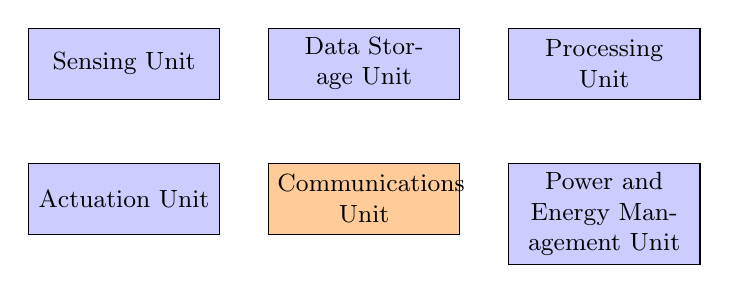
\begin{tikzpicture}[node distance=0.6cm, auto,
        block/.style={rectangle, draw, fill=blue!20, text width=2.2cm, text centered, minimum height=0.9cm, font=\small},
        highlight/.style={rectangle, draw, fill=orange!40, text width=2.2cm, text centered, minimum height=0.9cm, font=\small}]
        
        \node[block] (sense) {Sensing Unit};
        \node[block, right=of sense] (storage) {Data Storage Unit};
        \node[block, right=of storage] (proc) {Processing Unit};
        \node[block, below=0.8cm of sense] (act) {Actuation Unit};
        \node[highlight, below=0.8cm of storage] (comm) {Communications Unit};
        \node[block, below=0.8cm of proc] (power) {Power and Energy Management Unit};
        
    \end{tikzpicture}
    \end{center}
\end{frame}

%==============================================================================
% SLIDE 4: Part 2 Diagram
%==============================================================================
\begin{frame}{Part 2}
    \begin{center}
    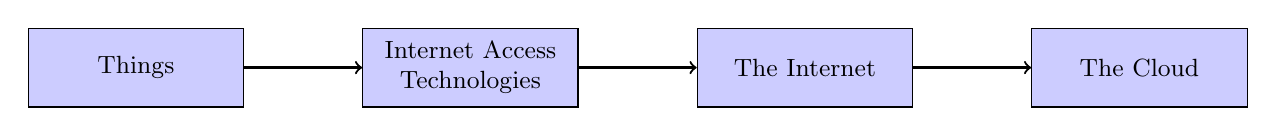
\begin{tikzpicture}[node distance=1.5cm, auto,
        block/.style={rectangle, draw, fill=blue!20, text width=2.5cm, text centered, minimum height=1cm, font=\small}]
        
        \node[block] (things) {Things};
        \node[block, right=of things] (access) {Internet Access Technologies};
        \node[block, right=of access] (internet) {The Internet};
        \node[block, right=of internet] (cloud) {The Cloud};
        
        \draw[->, thick] (things) -- (access);
        \draw[->, thick] (access) -- (internet);
        \draw[->, thick] (internet) -- (cloud);
    \end{tikzpicture}
    \end{center}
\end{frame}

%==============================================================================
% SLIDE 5: Outline (repeat)
%==============================================================================
\begin{frame}{Outline}
    \begin{itemize}
        \item \textbf{Part 1:} The Communications Unit
        \item \textbf{Part 2:} Protocols and Standards for the IoT
    \end{itemize}
\end{frame}

%==============================================================================
% SLIDE 6: Introduction
%==============================================================================
\begin{frame}{Introduction}
    \begin{itemize}
        \item In some applications, local data sensing and data processing are enough to make a decision and actuate
        \item In many other applications, communication is needed to:
        \begin{itemize}
            \item Enable information exchange between different sensors
            \item Enable information exchange with a remote sink
            \item Enable remote control
            \item \ldots
        \end{itemize}
    \end{itemize}
\end{frame}

%==============================================================================
% SLIDE 7: Introduction - Physics
%==============================================================================
\begin{frame}{Introduction}
    \textbf{There are different physics that support wireless communications:}
    \begin{itemize}
        \item \textbf{Electromagnetism}
        \begin{itemize}
            \item Near field communication through magnetic induction
            \item Radiowaves, microwaves, millimeter waves, terahertz waves
            \item Infrared, visible and ultra-violet optical signals
        \end{itemize}
        \item \textbf{Acoustics}
        \begin{itemize}
            \item Sound, ultra-sound signals
        \end{itemize}
        \item \textbf{Molecules}
        \begin{itemize}
            \item Ions, hormones, pheromones
        \end{itemize}
        \item \ldots
    \end{itemize}
\end{frame}

%==============================================================================
% SLIDE 8: Transceivers and Antennas
%==============================================================================
\begin{frame}{Transceivers and Antennas}
    \textbf{Transceiver = Transmitter + Receiver}
    \begin{itemize}
        \item The required hardware needed to generate (in transmission) and process (in reception) wireless signals
        \item Building blocks:
        \begin{itemize}
            \item Signal generators
            \item Modulators or Mixers (mix in the information)
            \item Amplifiers
            \item Filters
            \item \ldots
        \end{itemize}
    \end{itemize}
    
    \vspace{0.3cm}
    \textbf{Antenna:}
    \begin{itemize}
        \item The element that converts an electrical current in a propagating electromagnetic wave and vice versa
    \end{itemize}
\end{frame}

%==============================================================================
% SLIDE 9: The Communication Unit Block Diagram
%==============================================================================
\begin{frame}{The Communication Unit}
    \begin{center}
    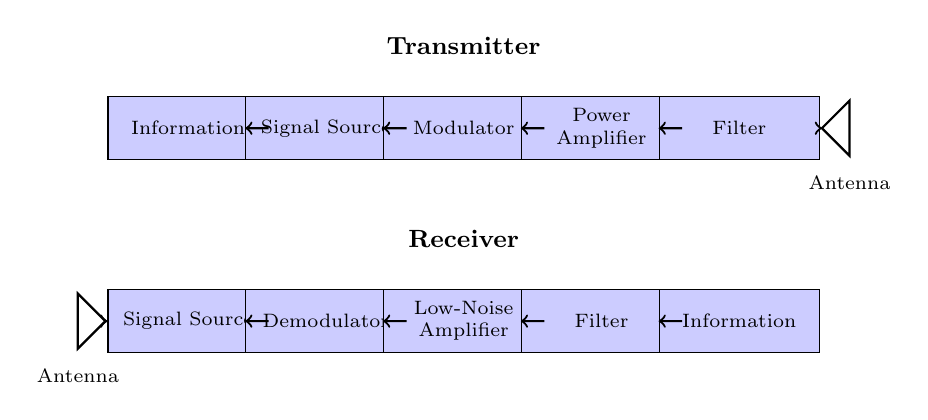
\begin{tikzpicture}[scale=0.7,
        block/.style={rectangle, draw, fill=blue!20, minimum width=2cm, minimum height=0.8cm, font=\scriptsize, text centered, text width=1.8cm}]
        
        % Transmitter
        \node[font=\small\bfseries] at (0, 3) {Transmitter};
        
        \node[block] (info1) at (-5, 1.5) {Information};
        \node[block] (source1) at (-2.5, 1.5) {Signal Source};
        \node[block] (mod) at (0, 1.5) {Modulator};
        \node[block] (pa) at (2.5, 1.5) {Power Amplifier};
        \node[block] (filt1) at (5, 1.5) {Filter};
        
        \draw[->, thick] (info1) -- (source1);
        \draw[->, thick] (source1) -- (mod);
        \draw[->, thick] (mod) -- (pa);
        \draw[->, thick] (pa) -- (filt1);
        
        % Antenna TX
        \draw[thick] (6.5, 1.5) -- (7, 2) -- (7, 1) -- cycle;
        \node[font=\scriptsize] at (7, 0.5) {Antenna};
        \draw[->, thick] (filt1) -- (6.5, 1.5);
        
        % Receiver
        \node[font=\small\bfseries] at (0, -0.5) {Receiver};
        
        \node[block] (source2) at (-5, -2) {Signal Source};
        \node[block] (demod) at (-2.5, -2) {Demodulator};
        \node[block] (lna) at (0, -2) {Low-Noise Amplifier};
        \node[block] (filt2) at (2.5, -2) {Filter};
        \node[block] (info2) at (5, -2) {Information};
        
        \draw[->, thick] (source2) -- (demod);
        \draw[->, thick] (demod) -- (lna);
        \draw[->, thick] (lna) -- (filt2);
        \draw[->, thick] (filt2) -- (info2);
        
        % Antenna RX
        \draw[thick] (-6.5, -2) -- (-7, -1.5) -- (-7, -2.5) -- cycle;
        \node[font=\scriptsize] at (-7, -3) {Antenna};
        \draw[->, thick] (-6.5, -2) -- (source2);
        
    \end{tikzpicture}
    \end{center}
\end{frame}

%==============================================================================
% SLIDE 10: Some Examples - Antennas
%==============================================================================
\begin{frame}{Some Examples}
    \begin{columns}
        \begin{column}{0.5\textwidth}
            \textbf{On-chip Antennas}
            \begin{itemize}
                \item Integrated directly on the silicon die
                \item Compact, low cost
                \item Limited gain and efficiency
            \end{itemize}
        \end{column}
        \begin{column}{0.5\textwidth}
            \textbf{Off-chip Antennas}
            \begin{itemize}
                \item External to the chip
                \item Better performance
                \item PCB trace, ceramic, wire antennas
            \end{itemize}
        \end{column}
    \end{columns}
\end{frame}

%==============================================================================
% SLIDE 11: Some (cooler) Examples
%==============================================================================
\begin{frame}{Some (cooler) Examples}
    \textbf{Paper-printed Electronics}
    \begin{itemize}
        \item Antennas and circuits printed on paper substrates
        \item Low cost, flexible, biodegradable
        \item Applications in disposable sensors, RFID tags
    \end{itemize}
\end{frame}

%==============================================================================
% SLIDE 12: Nano-transceivers and Nano-antennas
%==============================================================================
\begin{frame}{Nano-transceivers and Nano-antennas}
    \textbf{How could we make transceivers and antennas that are:}
    \begin{itemize}
        \item Smaller?
        \item Non-invasive?
        \item Non-perceptible?
    \end{itemize}
    
    \vspace{0.3cm}
    \textbf{By leveraging the tools provided by nanotechnology to:}
    \begin{itemize}
        \item Manipulate new materials, including graphene (remember Module 3)
        \item Leverage new physics, such as plasmonics
    \end{itemize}
    
    \vspace{0.3cm}
    \textbf{Applications:}
    \begin{itemize}
        \item The Internet of Nano-Things
    \end{itemize}
\end{frame}

%==============================================================================
% SLIDE 13: Transceiver and Antenna Specifications
%==============================================================================
\begin{frame}{Transceiver and Antenna Specifications}
    \begin{columns}
        \begin{column}{0.5\textwidth}
            \begin{itemize}
                \item Frequency band of operation
                \item Bandwidth
                \item Modulations
                \item Data-rate
                \item Transmission power
                \item Antenna gain
            \end{itemize}
        \end{column}
        \begin{column}{0.5\textwidth}
            \begin{itemize}
                \item Noise figure
                \item Sensitivity
                \item Communication distance / range
                \item Out of band emissions
                \item \ldots
            \end{itemize}
        \end{column}
    \end{columns}
    
    \vspace{0.5cm}
    \begin{block}{}
        Different communication and networking solutions will require different specifications.
        
        \textbf{More in Part 2}
    \end{block}
\end{frame}

%==============================================================================
% SLIDE 14: Transceiver States
%==============================================================================
\begin{frame}{Transceiver States}
    \textbf{Transceivers can be put into different operational states, typically:}
    \begin{itemize}
        \item \textbf{Transmit}
        \item \textbf{Receive}
        \item \textbf{Idle} -- ready to receive, but not doing so
        \begin{itemize}
            \item Some functions in hardware can be switched off, reducing energy consumption a little
        \end{itemize}
        \item \textbf{Sleep} -- significant parts of the transceiver are switched off
        \begin{itemize}
            \item Not able to immediately receive something
            \item Recovery time and startup energy to leave sleep state can be significant
        \end{itemize}
        \item \textbf{Research issue:} Wake-up receivers -- can be woken up via radio when in sleep state
    \end{itemize}
\end{frame}

%==============================================================================
% SLIDE 15: Energy Consumption
%==============================================================================
\begin{frame}{Energy Consumption}
    \begin{itemize}
        \item At this point, we have explained the key elements in the ``Things'' or embedded systems in IoT applications
        \item In many IoT applications, the ``Things'' are battery powered:
        \begin{itemize}
            \item Their batteries need to be periodically replaced or recharged
            \item Energy harvesting systems (e.g., solar, wind, motion) could be utilized
        \end{itemize}
        \item In all these cases, minimizing the power requirements and the energy consumption is a priority
        \item \textbf{Next, let's develop an energy model for ``Things'' in the IoT}
    \end{itemize}
\end{frame}

%==============================================================================
% SLIDE 16: Reminder - Units
%==============================================================================
\begin{frame}{Reminder}
    \begin{itemize}
        \item \textbf{Power} $\rightarrow$ Watts
        \item \textbf{Energy} $\rightarrow$ Joules (Watts $\times$ second)
        \item Energy = Power $\times$ Time
    \end{itemize}
    
    \vspace{0.3cm}
    \textbf{Logarithmic units:}
    \begin{itemize}
        \item Power in dBW = $10\log_{10}$(Power in Watts)
        \begin{itemize}
            \item E.g., 2 W = 3 dBW
        \end{itemize}
        \item Power in dBm (or dBmW) = $10\log_{10}$(Power in milliWatts)
        \begin{itemize}
            \item E.g., 1 mW = 0 dBm
        \end{itemize}
        \item Power Gain in dB = $10\log_{10}$(Gain unitless)
        \begin{itemize}
            \item E.g., 100$\times$ = 20 dB
        \end{itemize}
    \end{itemize}
\end{frame}

%==============================================================================
% SLIDE 17: Power & Energy Consumption Domains
%==============================================================================
\begin{frame}{Power \& Energy Consumption}
    \textbf{Power/Energy consumption in a sensor network can be divided into three domains:}
    \begin{itemize}
        \item Communication
        \item Data Processing (Computation)
        \item Sensing
    \end{itemize}
    
    \vspace{0.5cm}
    \begin{center}
    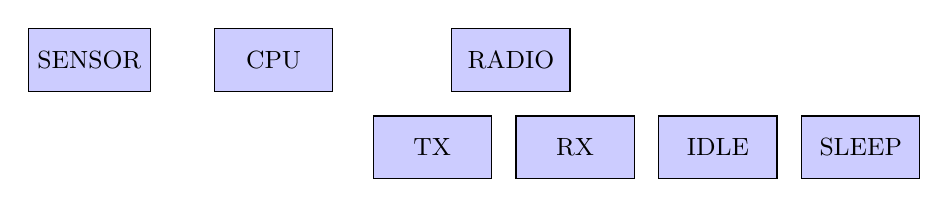
\begin{tikzpicture}[node distance=0.8cm,
        block/.style={rectangle, draw, fill=blue!20, minimum width=1.5cm, minimum height=0.8cm, font=\small}]
        
        \node[block] (sensor) {SENSOR};
        \node[block, right=of sensor] (cpu) {CPU};
        \node[block, right=1.5cm of cpu] (radio) {RADIO};
        
        \node[block, below=0.3cm of radio, xshift=-1cm] (tx) {TX};
        \node[block, right=0.3cm of tx] (rx) {RX};
        \node[block, right=0.3cm of rx] (idle) {IDLE};
        \node[block, right=0.3cm of idle] (sleep) {SLEEP};
        
    \end{tikzpicture}
    \end{center}
\end{frame}

%==============================================================================
% SLIDE 18: Energy Consumption in Communication
%==============================================================================
\begin{frame}{Energy Consumption in Communication}
    \begin{itemize}
        \item A ``Thing'' spends maximum energy in data communication (transmission and reception)
        \item For short range communication with low radiated power (e.g., 0 dBm), the transmission and reception energy costs are approximately the same
        \item Modern low power short range transceivers consume between \textbf{1 and 100 mW} of power when sending and receiving
        \item The energy consumption then depends on ``how long'' they are sending and receiving
        \item Transceiver circuitry has both \textbf{active} and \textbf{start-up} power/energy consumption
    \end{itemize}
\end{frame}

%==============================================================================
% SLIDE 19: Energy Consumption Formula
%==============================================================================
\begin{frame}{Energy Consumption in Communication}
    \[
    E_c = N_T[P_{te}(T_{on} + T_{st}) + P_O T_{on}] + N_R[P_{re}(R_{on} + R_{st})]
    \]
    
    \vspace{0.3cm}
    \begin{columns}
        \begin{column}{0.5\textwidth}
            \begin{itemize}
                \item $P_{te}$ is power consumed by transmitter
                \item $P_{re}$ is power consumed by receiver
                \item $P_O$ is output power of transmitter
                \item $T_{on}$ is transmitter ``on'' time
                \item $R_{on}$ is receiver ``on'' time
            \end{itemize}
        \end{column}
        \begin{column}{0.5\textwidth}
            \begin{itemize}
                \item $T_{st}$ is start-up time for transmitter
                \item $R_{st}$ is start-up time for receiver
                \item $N_T$ is the number of times transmitter is switched ``on''
                \item $N_R$ is the number of times receiver is switched ``on''
            \end{itemize}
        \end{column}
    \end{columns}
\end{frame}

%==============================================================================
% SLIDE 20: Energy Consumption - Parameters
%==============================================================================
\begin{frame}{Energy Consumption in Communication}
    \begin{itemize}
        \item $T_{on} = L / R$
        \begin{itemize}
            \item where $L$ is the packet size in bits and $R$ is the data rate in bits/second
        \end{itemize}
        \item The number of packets being sent and received, $N_T$ and $N_R$, depend on the protocols being used
        \item Low power radio transceiver has typical $P_{te}$ and $P_{re}$ values around \textbf{10 dBm} and $P_O$ close to \textbf{0 dBm}
    \end{itemize}
\end{frame}

%==============================================================================
% SLIDE 21: Start-up Power and Start-up Time
%==============================================================================
\begin{frame}{Start-up Power and Start-up Time}
    \begin{itemize}
        \item A transceiver spends time upon waking up from sleep mode, e.g., to ramp up phase locked loops or voltage-controlled oscillators (VCOs)
        \item During start-up time, no transmission or reception of data is possible
        \item ``Things'' often communicate in short data packets
        \item Start-up energy consumption (power $\times$ time) starts dominating as packet size is reduced
        \item It is inefficient to turn the transceiver ON and OFF because a large amount of energy is spent in turning the transceiver back ON each time
    \end{itemize}
\end{frame}

%==============================================================================
% SLIDE 22: Energy Consumption VS Packet Size
%==============================================================================
\begin{frame}{Energy Consumption VS Packet Size}
    \begin{columns}
        \begin{column}{0.5\textwidth}
            \begin{center}
                \textbf{Energy per packet [pJ]}
                
                \vspace{0.3cm}
                \begin{tikzpicture}[scale=0.6]
                    \draw[->] (0,0) -- (5,0) node[right, font=\footnotesize] {Packet Size [bits]};
                    \draw[->] (0,0) -- (0,4) node[above, font=\footnotesize] {$\times 10^4$};
                    \draw[thick, blue] (0.5,0.5) .. controls (1,1) and (2,2) .. (4.5,3.5);
                    \node[font=\tiny] at (1,-0.3) {$10^1$};
                    \node[font=\tiny] at (2.5,-0.3) {$10^2$};
                    \node[font=\tiny] at (4,-0.3) {$10^3$};
                \end{tikzpicture}
            \end{center}
        \end{column}
        \begin{column}{0.5\textwidth}
            \begin{center}
                \textbf{Energy per bit [pJ]}
                
                \vspace{0.3cm}
                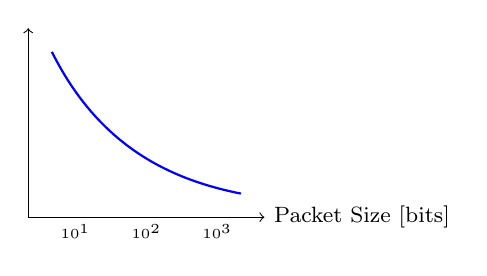
\begin{tikzpicture}[scale=0.6]
                    \draw[->] (0,0) -- (5,0) node[right, font=\footnotesize] {Packet Size [bits]};
                    \draw[->] (0,0) -- (0,4);
                    \draw[thick, blue] (0.5,3.5) .. controls (1.5,1.5) and (3,0.8) .. (4.5,0.5);
                    \node[font=\tiny] at (1,-0.3) {$10^1$};
                    \node[font=\tiny] at (2.5,-0.3) {$10^2$};
                    \node[font=\tiny] at (4,-0.3) {$10^3$};
                \end{tikzpicture}
            \end{center}
        \end{column}
    \end{columns}
    
    \vspace{0.3cm}
    \begin{itemize}
        \item As packet size is reduced, the energy consumption is dominated by the startup time on the order of hundreds of microseconds during which large amounts of energy are wasted
    \end{itemize}
\end{frame}

%==============================================================================
% SLIDE 23: Start Up and Sleep Mode
%==============================================================================
\begin{frame}{Start Up and Sleep Mode}
    \begin{itemize}
        \item The effect of the transceiver startup time will greatly depend on the type of MAC protocol used
        \item To reduce power consumption, it is desirable to have the transceiver in a sleep mode as often as possible
        \item However, constantly turning on and off the transceiver also consumes energy to bring it to readiness for transmission or reception
    \end{itemize}
    
    \vspace{0.5cm}
    \begin{center}
        \Large\textbf{Trade Off!}
    \end{center}
\end{frame}

%==============================================================================
% SLIDE 24: What about computation?
%==============================================================================
\begin{frame}{What about energy spent during computation?}
    \begin{center}
        \Large\textbf{?}
    \end{center}
\end{frame}

%==============================================================================
% SLIDE 25: Energy Consumption in Data Processing
%==============================================================================
\begin{frame}{Energy Consumption in Data Processing}
    \[
    E_p = N \cdot C \cdot V_{dd}^2 + V_{dd} \cdot I_O \cdot e^{\frac{n \cdot V_T}{f}}
    \]
    
    \begin{columns}
        \begin{column}{0.5\textwidth}
            \begin{itemize}
                \item $N$ is the number of clock cycles per task
                \item $C$ is the average capacitance switched per cycle
                \item $V_{dd}$ is the supply voltage
                \item $V_T$ is the thermal voltage
            \end{itemize}
        \end{column}
        \begin{column}{0.5\textwidth}
            \begin{itemize}
                \item $I_O$ is output current
                \item $f$ is the switching frequency
                \item $n$ is the ideality factor
            \end{itemize}
            
            \vspace{0.3cm}
            \small
            \textit{This term represents leakage current. In general, leakage currents account for about 10\% of the total energy dissipation.}
        \end{column}
    \end{columns}
    
    \vspace{0.3cm}
    \textbf{Remember from Module 3:} All these parameters depend on your transistor technology
\end{frame}

%==============================================================================
% SLIDE 26: Energy Consumption - Computation vs Communication
%==============================================================================
\begin{frame}{Energy Consumption in Data Processing}
    \begin{itemize}
        \item The energy consumed in data processing is often \textbf{much less} than the energy consumed in communication
        \item \textbf{Example:}
        \begin{itemize}
            \item Assumptions:
            \begin{itemize}
                \item Traditional low-power radio operating at 1-2 GHz
                \item Rayleigh Fading wireless channel with losses depending with the fourth power of distance (More in Module 4, Part 2)
            \end{itemize}
            \item Result:
            \begin{itemize}
                \item Energy cost of transmitting 1 kilobyte (kB) at a distance of 100 meters (m) is approximately equal to executing \textbf{3 million instructions} by a 100 million instructions per second processor
            \end{itemize}
        \end{itemize}
        \item \textbf{Performing local data processing is crucial to minimize the total energy consumption of the system!}
        \item That's the same reason why we try to perform as much processing as possible close to the data source $\rightarrow$ \textbf{Edge Computing}
    \end{itemize}
\end{frame}

%==============================================================================
% SLIDE 27: Some Examples - MCUs
%==============================================================================
\begin{frame}{Some Examples}
    \textbf{Commercial Microcontrollers}
    
    \vspace{0.3cm}
    \textbf{TI MSP 430} (@ 1 MHz, 3V):
    \begin{itemize}
        \item Fully operational: \textbf{1.2 mW}
        \item Deepest sleep mode: \textbf{0.3 $\mu$W}
        \begin{itemize}
            \item Only woken up by external interrupts (not even timer is running anymore)
        \end{itemize}
    \end{itemize}
    
    \vspace{0.3cm}
    \textbf{Atmel ATMega}:
    \begin{itemize}
        \item Operational mode: \textbf{15 mW} active, \textbf{6 mW} idle
        \item Sleep mode: \textbf{75 $\mu$W}
    \end{itemize}
\end{frame}

%==============================================================================
% SLIDE 28: Dynamic Voltage Scaling
%==============================================================================
\begin{frame}{Alternative: Dynamic Voltage Scaling}
    \textbf{Rationale:}
    \begin{itemize}
        \item Power consumption $P$ depends on:
        \begin{itemize}
            \item Clock frequency
            \item Square of supply voltage
        \end{itemize}
        \item $P \sim f \cdot V^2$
        \item Lower clock allows lower supply voltage
        \item \textbf{But:} execution takes longer
    \end{itemize}
\end{frame}

%==============================================================================
% SLIDE 29: Memory Power Consumption
%==============================================================================
\begin{frame}{Memory Power Consumption}
    \begin{itemize}
        \item \textbf{Crucial part:} FLASH memory
        \item Power for RAM almost negligible
        \item FLASH writing/erasing is expensive
    \end{itemize}
    
    \vspace{0.3cm}
    \textbf{Example: FLASH on Mica motes}
    \begin{itemize}
        \item Reading: $\approx$ 1.1 nAh per byte
        \item Writing: $\approx$ 83.3 nAh per byte
    \end{itemize}
    
    \vspace{0.3cm}
    \small
    \textit{Ah = Ampere hour}\\
    \textit{Multiply by voltage V in volts to obtain Watt hour or Wh}\\
    \textit{Multiply by 3600 seconds/hour to obtain Watt second = Joule}
\end{frame}

%==============================================================================
% SLIDE 30: Computation VS Communication Cost
%==============================================================================
\begin{frame}{Computation VS Communication Cost}
    \textbf{Tradeoff?}
    \begin{itemize}
        \item Directly comparing computation/communication energy cost is not easy
        \item It really depends on the technology being used:
        \begin{itemize}
            \item 900 MHz RF system
            \item 2.4 GHz WiFi/Bluetooth System
            \item 3.1-10.6 GHz Ultra-wide-band System
            \item 60 GHz mmWave system
            \item \ldots
        \end{itemize}
        \item Besides the amplifiers in your transceiver, the digital to analog and the analog to digital converters (DACs and ADCs), i.e., the interface between analog signals and your digital computer, are one of the most energy consuming elements
    \end{itemize}
\end{frame}

%==============================================================================
% SLIDE 31: Let's put everything together
%==============================================================================
\begin{frame}{Let's put everything together:}
    \begin{center}
        \Large\textbf{A simple energy model}
    \end{center}
\end{frame}

%==============================================================================
% SLIDE 32: A Simple Energy Model
%==============================================================================
\begin{frame}{A Simple Energy Model}
    \textbf{Consider that a ``Thing'' is only operating in transmit and receive modes with the following assumptions:}
    
    \vspace{0.3cm}
    \begin{itemize}
        \item Energy to run circuitry:
        \begin{itemize}
            \item $E_{elec}$ = 50 nJ/bit
        \end{itemize}
        \item Energy for radio transmission:
        \begin{itemize}
            \item $E_{amp}$ = 100 pJ/bit/m$^2$
        \end{itemize}
        \item Energy for sending $k$ bits over distance $D$:
        \begin{itemize}
            \item $E_{Tx}(k,D) = E_{elec} \cdot k + E_{amp} \cdot k \cdot D^2$
        \end{itemize}
        \item Energy for receiving $k$ bits:
        \begin{itemize}
            \item $E_{Rx}(k) = E_{elec} \cdot k$
        \end{itemize}
    \end{itemize}
\end{frame}

%==============================================================================
% SLIDE 33: A Simple Energy Model - Diagram
%==============================================================================
\begin{frame}{A Simple Energy Model}
    \begin{columns}
        \begin{column}{0.5\textwidth}
            $E_{Tx}(k,D) = E_{Tx-elec}(k) + E_{Tx-amp}(k,D)$
            
            $E_{Tx}(k,D) = E_{elec} \cdot k + E_{amp} \cdot k \cdot D^2$
            
            \vspace{0.5cm}
            $E_{Rx}(k) = E_{Rx-elec}(k)$
            
            $E_{Rx}(k) = E_{elec} \cdot k$
        \end{column}
        \begin{column}{0.5\textwidth}
            \begin{table}
                \centering
                \footnotesize
                \begin{tabular}{@{}lc@{}}
                    \toprule
                    \textbf{Operation} & \textbf{Energy} \\
                    \midrule
                    TX/RX Electronics & 50 nJ/bit \\
                    TX Amplifier & 100 pJ/bit/m$^2$ \\
                    \bottomrule
                \end{tabular}
            \end{table}
        \end{column}
    \end{columns}
    
    \vspace{0.5cm}
    \begin{center}
    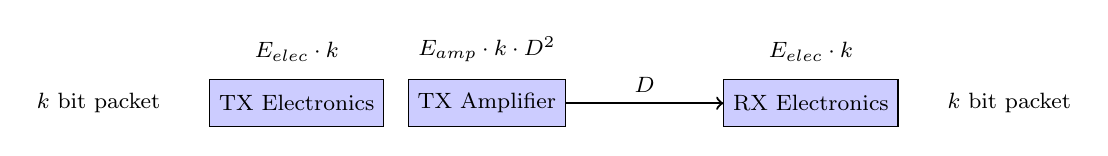
\begin{tikzpicture}[scale=0.8, node distance=0.5cm,
        block/.style={rectangle, draw, fill=blue!20, minimum width=1.5cm, minimum height=0.6cm, font=\footnotesize}]
        
        \node[block] (txelec) {TX Electronics};
        \node[block, right=0.3cm of txelec] (txamp) {TX Amplifier};
        \node[font=\footnotesize, above=0.1cm of txelec] {$E_{elec} \cdot k$};
        \node[font=\footnotesize, above=0.1cm of txamp] {$E_{amp} \cdot k \cdot D^2$};
        
        \node[font=\footnotesize, left=0.5cm of txelec] {$k$ bit packet};
        
        \node[block, right=2cm of txamp] (rxelec) {RX Electronics};
        \node[font=\footnotesize, above=0.1cm of rxelec] {$E_{elec} \cdot k$};
        \node[font=\footnotesize, right=0.5cm of rxelec] {$k$ bit packet};
        
        \draw[->, thick] (txamp) -- node[above, font=\footnotesize] {$D$} (rxelec);
        
    \end{tikzpicture}
    \end{center}
\end{frame}

%==============================================================================
% SLIDE 34: Example Using the Energy Model
%==============================================================================
\begin{frame}{Example Using the Energy Model}
    \textbf{What is the energy consumption if 1 Mbit of information is transferred from the source to the sink where the source and sink are separated by 100 meters and the broadcast radius of each node is 5 meters? Assume the neighbor nodes are overhearing each other's broadcast.}
    
    \vspace{0.5cm}
    \begin{center}
    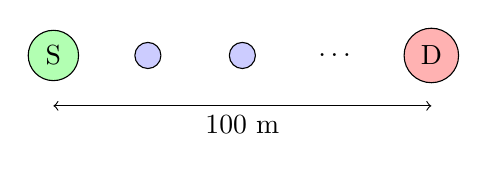
\begin{tikzpicture}[scale=0.8]
        \node[circle, draw, fill=green!30] (s) at (0,0) {S};
        \node[circle, draw, fill=blue!20] (n1) at (1.5,0) {};
        \node[circle, draw, fill=blue!20] (n2) at (3,0) {};
        \node at (4.5,0) {\ldots};
        \node[circle, draw, fill=red!30] (d) at (6,0) {D};
        
        \draw[<->] (0,-0.8) -- node[below] {100 m} (6,-0.8);
    \end{tikzpicture}
    \end{center}
\end{frame}

%==============================================================================
% SLIDE 35: Conclusion
%==============================================================================
\begin{frame}{Conclusion}
    \begin{itemize}
        \item Energy is an extremely important factor in the design of your wireless internet of things
        \item It is extremely device and application dependent:
        \begin{itemize}
            \item What type of transceiver do you have?
            \item What type of processor do you have?
            \item How often are these used?
        \end{itemize}
        \item All these also depend on the communication and networking protocols
        \item \textbf{That's the focus of Module 4 - Part 2}
    \end{itemize}
\end{frame}

%==============================================================================
% SLIDE 36: Questions
%==============================================================================
\begin{frame}{Questions?}
    \begin{center}
        \Huge\textbf{?}
    \end{center}
\end{frame}

%==============================================================================
% References
%==============================================================================
\begin{frame}[allowframebreaks]{References}
    \printbibliography
\end{frame}

\end{document}
